\documentclass[11pt]{article}
\usepackage[spanish]{babel}
\usepackage{amsmath}
\usepackage{amssymb}
\usepackage{graphicx}
\graphicspath{ {./images/}, {~/Apunte/images/} }
\usepackage[utf8]{inputenc}
\usepackage[T1]{fontenc}
\usepackage[margin=1in]{geometry}
\usepackage{fancyhdr}
\usepackage{hyperref}

\hypersetup{
    pdftitle={Reporte Post-Laboratorio 3: Planillas de Cálculo 3},
    pdfauthor={Felipe Colli Olea},
    colorlinks=true,
    linkcolor=black,
    urlcolor=cyan
}

\pagestyle{fancy}
\fancyhf{}
\fancyfoot[C]{\footnotesize Felipe Colli, Todos los Derechos Reservados}
\fancyfoot[R]{\thepage}
\renewcommand{\headrulewidth}{0pt}

\title{Reporte Post-Laboratorio: Planillas de Cálculo 3 \\ \large{Herramientas Computacionales para Ingeniería y Ciencias}}
\author{Felipe Colli Olea}
\date{\today}

\begin{document}

\maketitle
\thispagestyle{fancy}

% ------------------------------------------------------------------------------
% INTRODUCCIÓN
% ------------------------------------------------------------------------------
\section{Introducción}

El presente informe expone el trabajo desarrollado durante el tercer y último laboratorio de la unidad de planillas de cálculo. Esta actividad subió bastante el nivel respecto a las sesiones anteriores, ya que nos enfrentamos a una base de datos mucho más grande: el registro histórico de contaminación por PM 2,5 en Santiago a lo largo de 16 años.

El objetivo central del laboratorio fue aprender a filtrar, resumir y graficar esta gran cantidad de datos para obtener información útil, utilizando funciones lógicas complejas y descubriendo la utilidad de las Tablas Dinámicas.

% ------------------------------------------------------------------------------
% DESARROLLO Y TRABAJOS REALIZADOS
% ------------------------------------------------------------------------------
\section{Desarrollo de Actividades}

\subsection{Procesamiento de Datos y Gráficos}
El primer paso consistió en preparar la base de datos y visualizarla.

\begin{itemize}
	\item \textbf{Gráficos de Líneas:} Se graficó el registro de contaminación diario. Al ser más de 5800 datos, el gráfico resultante es bastante denso, por lo que fue importante ponerle títulos y leyendas claras para que se entendiera qué estábamos viendo.

	\item \textbf{Columnas Auxiliares:} Para facilitar el cálculo posterior, agregamos dos columnas. Una usando la función \texttt{=AÑO()} para extraer el año de cada fecha. La otra fue una columna condicional usando \texttt{=SI()}, donde le indicamos al programa que pusiera un \texttt{1} si el nivel de contaminación superaba la norma y un \texttt{0} si estaba dentro de lo permitido. Esto fue clave para poder sumar los días críticos más adelante.
\end{itemize}

% Placeholder para la imagen de los gráficos
\begin{figure}[h]
	\centering
	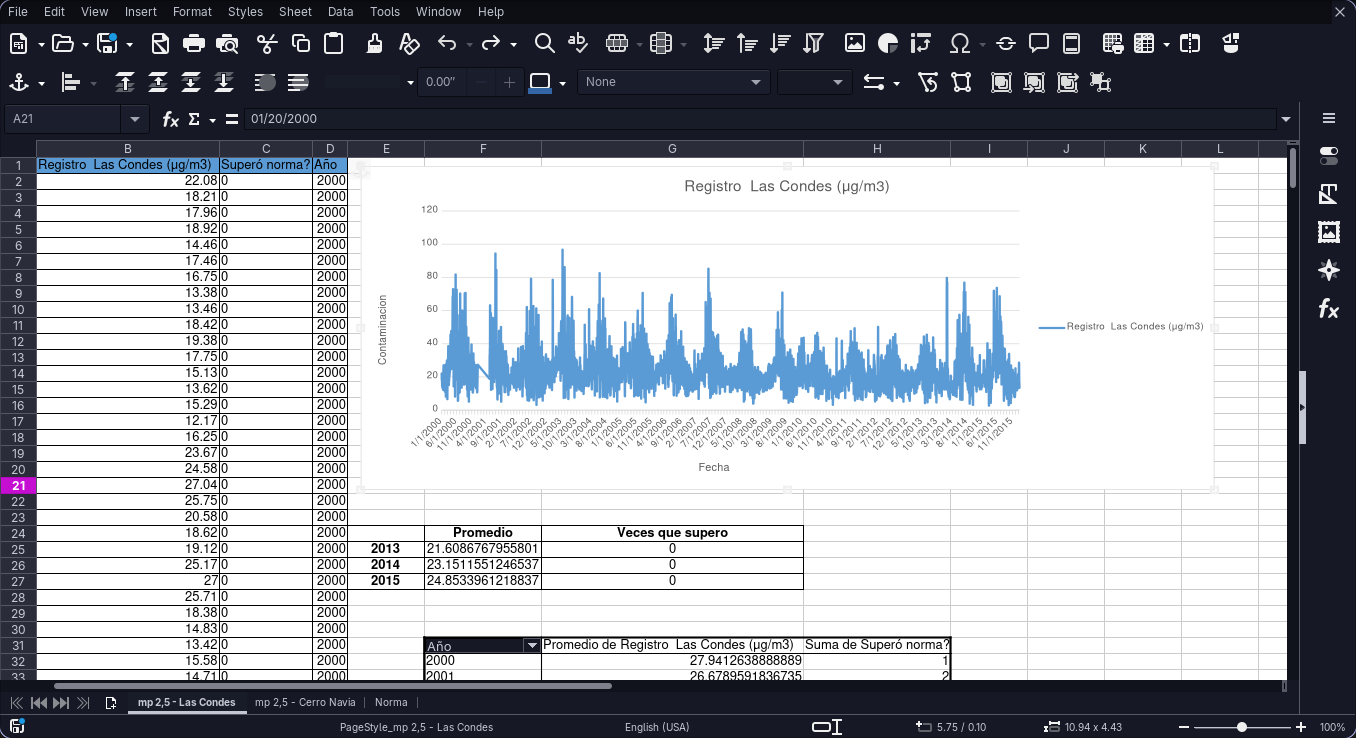
\includegraphics[width=0.8\textwidth]{grafico.png}
	\caption{Visualización histórica de los niveles de PM 2,5.}
\end{figure}

\subsection{Fórmulas vs. Tablas Dinámicas}
La parte central del laboratorio nos pidió calcular el promedio de contaminación y los días que se superó la norma para los años 2013, 2014 y 2015. Esto lo hicimos de dos maneras para comparar:

\begin{itemize}
	\item \textbf{Con Fórmulas largas:} Utilizamos \texttt{PROMEDIO.SI.CONJUNTO()} y \texttt{CONTAR.SI.CONJUNTO()}. Aquí tuvimos que seleccionar cuidadosamente los rangos y poner múltiples criterios (por ejemplo, que el año fuera igual a 2013).

	\item \textbf{Con Tablas Dinámicas:} Luego hicimos exactamente lo mismo pero insertando una Tabla Dinámica. Arrastramos el "Año" a las filas y le pedimos que nos diera el promedio de los registros y la suma de la columna auxiliar que creamos antes. El resultado fue idéntico pero se logró en una fracción del tiempo.
\end{itemize}

% Placeholder para la imagen de las tablas
\begin{figure}[h]
	\centering
	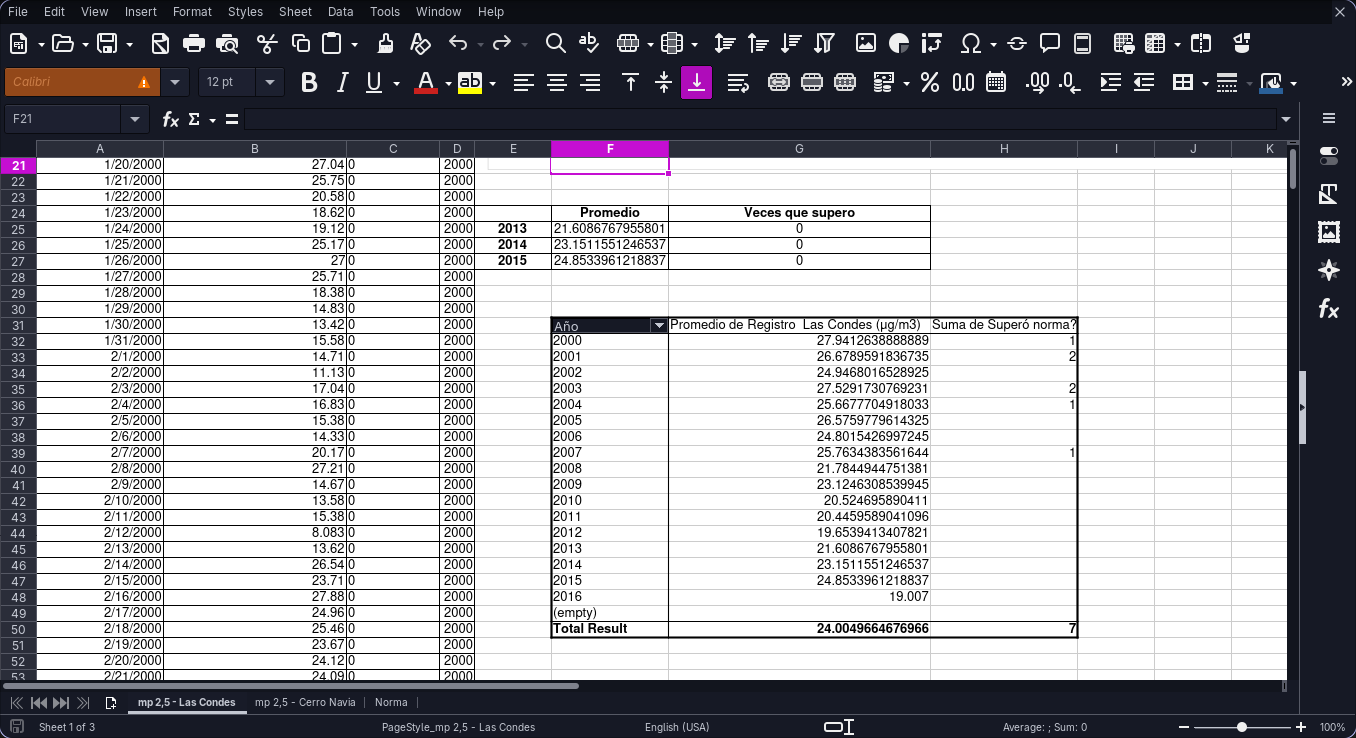
\includegraphics[width=0.8\textwidth]{dinamica.png}
	\caption{Comparativa entre el uso de fórmulas .SI.CONJUNTO y Tablas Dinámicas.}
\end{figure}

\vspace{0.5cm}
\noindent\textit{\textbf{Nota sobre la evidencia visual:} Al igual que en las sesiones previas, el trabajo en parejas se desarrolló en los computadores de la facultad (Windows/Excel). Sin embargo, para mantener la homogeneidad de mi flujo de trabajo en \LaTeX{} bajo Arch Linux, la evidencia de este informe fue capturada renderizando el archivo \texttt{.xlsx} original en mi computador usando \texttt{LibreOffice Calc}.}

\newpage
% ------------------------------------------------------------------------------
% REFLEXIONES Y DIFICULTADES
% ------------------------------------------------------------------------------
\section{Reflexiones y Dificultades}

La principal dificultad de este laboratorio fue lidiar con las funciones \texttt{.SI.CONJUNTO}. Escribir fórmulas tan largas en la pequeña barra de Excel es muy propenso a errores. A diferencia de un entorno de programación donde uno puede tabular el código e identificar los paréntesis fácilmente, en la planilla es fácil equivocarse seleccionando un rango o olvidando fijar una celda, lo que te obliga a revisar todo desde cero.

Además, trabajar con casi 6000 filas hizo que los gráficos se sintieran un poco lentos al momento de hacer zoom o mover la hoja, lo que demuestra que herramientas ofimáticas como Excel empiezan a tener límites de rendimiento cuando la cantidad de datos crece.

Por último, el contraste entre usar fórmulas y usar la Tabla Dinámica fue revelador. La Tabla Dinámica simplificó enormemente el trabajo, evitando el riesgo de equivocarse al tipear, lo que la hace una herramienta mucho más segura para resumir datos.

% ------------------------------------------------------------------------------
% CONCLUSIONES
% ------------------------------------------------------------------------------
\section{Conclusiones}

Este laboratorio fue un excelente cierre para la unidad. Me permitió entender que, si bien Excel puede volverse tedioso cuando se intenta usar como un lenguaje de programación a base de fórmulas anidadas interminables, tiene herramientas integradas muy potentes.

Las Tablas Dinámicas resultaron ser el gran descubrimiento de la clase. Entender cómo agrupar, promediar y sumar grandes volúmenes de datos con un par de clics es una habilidad muy práctica para el futuro. Aunque mi preferencia personal sigue siendo el control absoluto que te da el código puro y el entorno de terminal para procesar datos, reconozco que para sacar resúmenes rápidos y visuales, las planillas de cálculo son una herramienta que todo estudiante de ingeniería debe manejar.

\end{document}
